\documentclass[12pt, twoside]{article}
\usepackage{jmlda}
\newcommand{\hdir}{.}
\usepackage[utf8]{inputenc}
\usepackage[english,russian]{babel}
\usepackage{graphicx}
\newcommand{\real}{\mathbb{R}}
\newcommand{\nat}{\mathbb{N}}
\newcommand{\integ}{\mathbb{Z}}
\usepackage{bm}
\usepackage{multicol}
\usepackage{graphicx}
\graphicspath{{img/}}
\DeclareGraphicsExtensions{.pdf,.png,.jpg}
%\usepackage[round]{natbib}
%\usepackage[
%backend=biber,
%style=alphabetic,
%sorting=ynt
%]{biblatex}

%\addbibresource{Kulagin.bib}



\begin{document}

%\nocite{*}

\title
    [Шаблон статьи для публикации] % краткое название; не нужно, если полное название влезает в~колонтитул
    {Построение метода динамического выравнивания многомерных временных рядов, устойчивого к локальным колебаниям сигнала.}
\author
    [И.\,О.~Автор] % список авторов (не более трех) для колонтитула; не нужен, если основной список влезает в колонтитул
    {П.\,А.~Кулагин, Г.\,И.~Моргачев, А.\,В.~Гончаров, В.\,В~Стрижов} % основной список авторов, выводимый в оглавление
    [И.\,О.~Автор$^1$, И.\,О.~Соавтор$^2$, И.\,О.~Фамилия$^{1,2}$] % список авторов, выводимый в заголовок; не нужен, если он не отличается от основного
\email
    {kulagin.pyoter@mail.ru; co-author@site.ru;  co-author@site.ru}
\thanks
    {Работа выполнена при
     %частичной
     финансовой поддержке РФФИ, проекты \No\ \No 00-00-00000 и 00-00-00001.}
\organization
    {$^1$Организация, адрес; $^2$Организация, адрес}
\abstract
    {Данная работа посвящена построению эффективного алгоритма динамического выравнивания многомерных временных рядов. Для решения данной задачи предлагается использовать функцию расстояния DTW между двумя многомерными временными рядами, согласно которому выравниваются две оси времени, при этом внутри функционала DTW выбирается расстояние между i-м и j-м измерениями такое, что оно устойчиво к локальным “сдвигам” сигнала. В качестве решения будет рассмотрено более продвинутое, основанное на DTW между парой измерений. Для проверки корректности используются как и реальные данные, например измерения активность мозга обезьян, так и искусственно сгенерированные, например движение сигнала в пространстве по часовой и против часовой стрелки.
	
\bigskip
\noindent
\textbf{Ключевые слова}: \emph {многомерные временные ряды; DTW; динамическое выравнивание.}
}

\maketitle
\linenumbers

\section{Введение}

В данной работе исследуется проблема динамического выравнивания многомерных временных рядов, устойчивого к локальным колебаниям сигнала.
Временной ряд -  собранный в разные моменты времени статистический материал о значении каких-либо параметров (в простейшем случае одного исследуемого процесса). В данном случае рассматривается многомерный случай.

Необходимость сравнивать 2 временных ряда на схожесть возникает из практических задач таких как классификация геномных сигналов~\cite{Skutkova2013}, распознавание жестов~\cite{Holt2007}.  


При этом необходимо учитывать, что в таких задачах как ... возникает необходимо учитывать, что близость временных рядов не ограничивается сдвигами по времени, а также присутствует  расположениям сигналов.

Для сравнения определения расстояния между временными рядами будет использовать известный алгоритм DTW~\cite{Keogh01derivativedynamic}~\cite{SalvadorC07}, однако возникает проблема определения расстояния между сигналами в этом алгоритме.

Базовое решение задачи с помощью метрики L2 расстояния между рядами~\cite{Sanguasat2012} не всегда оказывается эффективным. Таким примером являются 2 временных ряда, полученные при близком расположении датчиков с сигналами, которые могут зафиксировать один и тот же пик. Полученный пик окажет большое влияние на значение метрики L2.

Напротив, использование известного алгоритма DTW, но уже в многомерном случае позволит обойти проблему малого расстояния между датчиками, как более частный метод для решения конкретного типа задач.

Итак, в данной работе рассматриваются 2 варианта расстояния между сигналами L2 и DTW, выравнивание по временной оси будет сглаживать DTW.

Полученные алгоритмы тестировались на реальных данных и искуственно сгенерированных. Полученные результаты показали преимущество использования попарного DTW алгоритма.


\section{Постановка задачи.}

Рассматривается алгоритм решения задачи динамического выравнивания многомерных рядов.

Задача классификации временных рядов имеет вид.

Пусть X - множество временных рядов, Y - множество меток классов.

$\forall x \in X x \in \mathbb{R^K}$

Рассматриваем $Y = \{0, 1\}$,  $|Y| = 2$, то есть задачу бинарной классификации.

Предполагается существование зависимости $f: X \rightarrow Y$

Задача заключается в поиске оптимального алгоритма из семейства $A = \{a_{\alpha}\}$, предсказывающего класс из множества Y.

Семейство алгоритмов задаётся 

Пусть $X^n = \{X_1, X_2 \dots X_n\}$ - обучающая выборка из временных рядов, $Y^n = \{Y_1, Y_2 \dots Y_n\}$ - метки классов.

В качестве семейства алгоритмов классификации будем использовать метод k ближайших соседей с некоторой

метрикой $\rho$ - расстоянием между 2 временными рядами.

Оптимизируемый функционал $accuracy = \frac{TP + TN}{TP + TN + FP + FN}$

Хотим предоставить $\rho = \argmax(accuracy)$ - как можно ближе к оптимальному.

При этом считаем, что данные представляют собой не произвольной временной ряд, а временной ряд

у которого известны местоположения датчиков в пространстве, а сигнал может искажаться и улавливаться соседними датчиками.


\section{Рассматриваемые метрики}

В данной работе будут работе будут рассматриваться и сравниваться 2 метрики, которые будут введены в этом разделе.

Введём функцию расстояния между 2 временными рядами с помощью алгоритма DTW.

$D(i, j) = d(i, j) + min(D(i - 1, j), D(i, j - 1), D(i - 1, j - 1))$

$d(i, j)$ - расстояние между парой сигналов. Определяется 2 разными способами.

1) L2 - метрика.

$d(i, j) = \Sigma_{k = 1}^K(X(i, k) - X(j, k))^2$

2) DTW - расстояние.

$d(i, j, k, t) = (X(i, k) - X(j, t)) ^ 2 + min(d(i, j, k - 1, t), d(i, j, k, t - 1), d(i, j, k - 1, t - 1))$

$d(i, j) := d(i, j, K, K)$

Будем исследовать метрики L2 и DTW, задающие различные варианты расстояний между сигналами. 

Пример выравнивания для L2 и DTW временного ряда с 3 измерителями.

Для L2

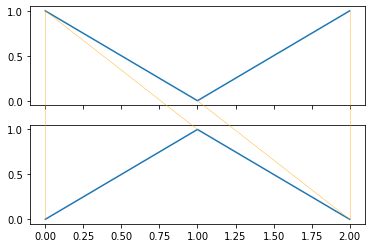
\includegraphics{sample11}

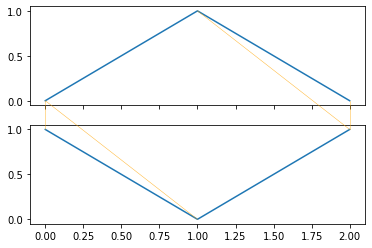
\includegraphics{sample12}

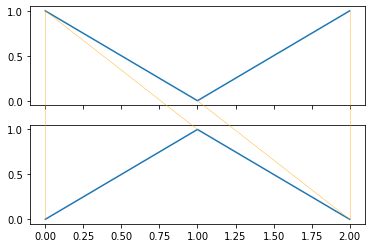
\includegraphics{sample13}

И для DTW

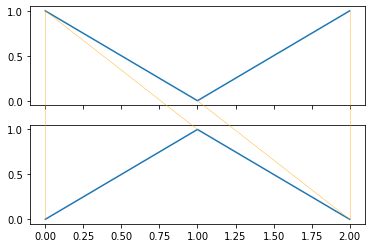
\includegraphics{sample21}

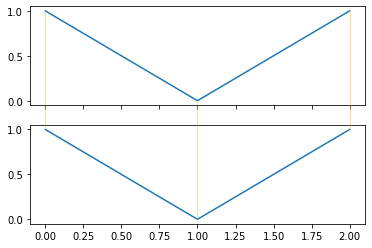
\includegraphics{sample22}

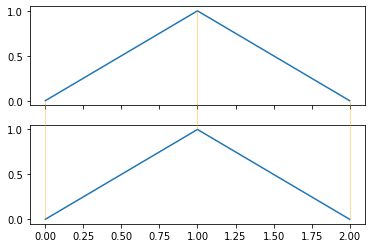
\includegraphics{sample23}

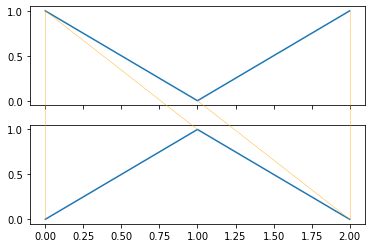
\includegraphics{sample24}

%А также многомерные сигналы, которые которые замерялись на поверхности мозга обезьян. Датчики при этом находились на небольшом расстояниии друг от друга. 


\section{Вычислительный эксперимент}

\subsection{Цель эксперимента}

Данный преследует 3 цели.

1) Найти примеры временных рядов, удовлетворяющих свойству пространственности измерителей.

2) Измерить время работы 2 методов выравнивания.

3) Решить задачу классификации для многомерных временных рядов в предположении о данных сделанное ранее и сравнить точность предсказания.

2 пункт важен, так как время работы алгоритмов отличается довольно сильно.

\subsection{Эксперимент на исккусственных данных}


Рассмотрим примеры данных, полученные искусственной генерацией.

1) Сигнал перемещается по часовой стрелке вокруг одного набора датчиков и против часовой стрелки для другого набора датчиков.

Более формально, рассматриваем 2 временных ряда $t_1$  и $t_2$ длины $k$ и размера $k$.

Условимся все индексы векторов нумеровать с 0.

Тогда для i измерения в ряде $t_1$ i сигнал будет равен 1, а остальные нули.

В ряде $t_2$ единицы будут стоять на местах $k - i - 1$ для $i$ измерения.


На графике показано движение сигнала для 2 временных рядов.

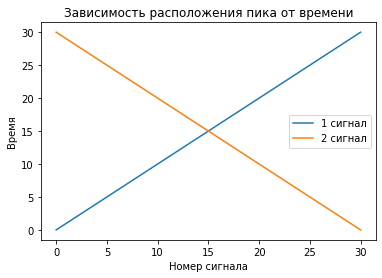
\includegraphics{rev_signal}

2) Сигнал перемещается в 2 раза быстрее вокруг одного из наборов датчиков.

Более формально, рассматриваем 2 временных ряда $t_1$  и $t_2$ длины $k$ и размера $k$.

Условимся все индексы векторов нумеровать с 0.

Тогда для i измерения в ряде $t_1$ i сигнал будет равен 1, а остальные нули.

В ряде $t_2$ единицы будут стоять на местах $(2 * i + 1) mod k$ для $i$ измерения.

Пример хорошо используется только для нечётного $k$.

На графике также показано движение сигнала для 2 временных рядов.

На графике показано движение сигнала для 2 временных рядов.

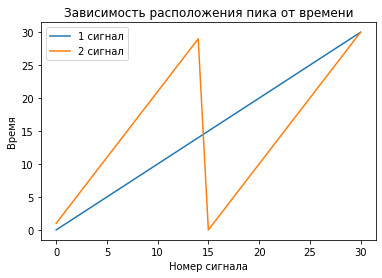
\includegraphics{up}


Если измерить их по метрике L2 и DTW, то в 1 случае получатся значения 60 и 4,

а во втором - 60 и 2. То есть алгоритм DTW имеет большую необходимость в этом случае.


\subsection{Временной эксперимент}

Временной эксперимент имеет также имеет огромное значение, так как использование алгоритма
может быть затруднено в силу низкой скорости обработки, и соответственно малым количеством данных для обучения.

Эксперимент со временем запускался на данных с 

размерностью сигнала: 3

количество измерений: 50

количеством временных рядов: 20

В итоге зависимость среднего времени измерения расстояния (использовалось 100 случайных временных рядов) от количества измерений

представлена на следующем графике.

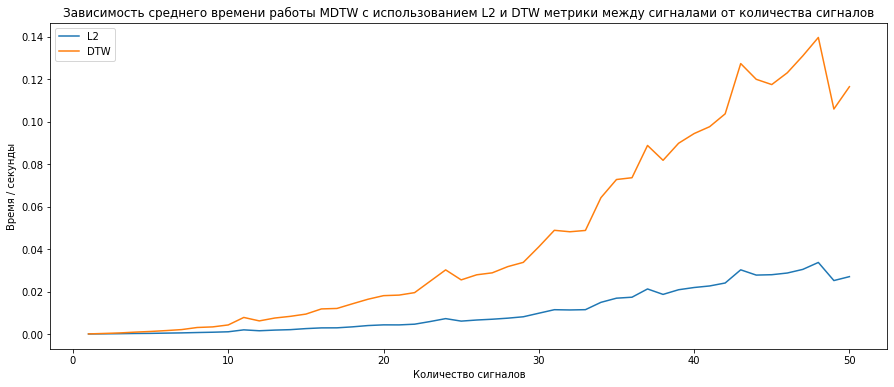
\includegraphics[scale=0.5]{time}

Можно сделать вывод, что DTW работает медленнее и не на всех данных следует его использовать.

\section{Заключение}

Было продемонстрировано значение метрики DTW для поиска расстояний между сигналами

в многомерном случае. Однако затрачиваемое время на порядок медленнее L2 алгоритма.

Поэтому стоит использовать $L2$ или DTW в зависимости от задачи и временных ограничений.


\nocite{*}
 
\bibliographystyle{unsrt}
\bibliography{Kulagin}

\end{document}